%-------------------------------------------------------------------------------
%	PACKAGES AND OTHER DOCUMENT CONFIGURATIONS
%-------------------------------------------------------------------------------

\documentclass[11pt]{article}

% Packages
% Packages

% \usepackage{fancyhdr} % Required for custom headers
% \usepackage{lastpage} % Required to determine the last page for the footer
% \usepackage{extramarks} % Required for headers and footers
% \usepackage[usenames,dvipsnames]{color} % Required for custom colors
\usepackage{graphicx} % Required to insert images
% \usepackage{listings} % Required for insertion of code
% \usepackage{courier} % Required for the courier font
% \usepackage{dsfont} % For special math characters
% \usepackage{verbatim}

%\usepackage{amsmath, amssymb, bm} % For matrix notation
\usepackage[english]{babel}
\usepackage[paperwidth=8.5in,paperheight=11in,margin=1.0in]{geometry}
\usepackage{listings}
\usepackage{hyperref}
%\usepackage[cmex10]{amsmath, bm}
\usepackage{amsmath, bm}
\usepackage{blkarray}








% formatting
\pdfcompresslevel0

% ==============================================================================
% PYTHON
% ==============================================================================
\usepackage[utf8]{inputenc}

% Default fixed font does not support bold face
\DeclareFixedFont{\ttb}{T1}{txtt}{bx}{n}{12} % for bold
\DeclareFixedFont{\ttm}{T1}{txtt}{m}{n}{12}  % for normal

% Custom colors
\usepackage{color}
\definecolor{deepblue}{rgb}{0,0,0.5}
\definecolor{deepred}{rgb}{0.6,0,0}
\definecolor{deepgreen}{rgb}{0,0.5,0}

\usepackage{listings}

% Python style for highlighting
\newcommand\pythonstyle{\lstset{
language=Python,
basicstyle=\ttm,
otherkeywords={self},             % Add keywords here
keywordstyle=\ttb\color{deepblue},
emph={MyClass,__init__},          % Custom highlighting
emphstyle=\ttb\color{deepred},    % Custom highlighting style
stringstyle=\color{deepgreen},
frame=tb,                         % Any extra options here
showstringspaces=false,            % 
breaklines=true
}}


% Python environment
\lstnewenvironment{python}[1][]
{\pythonstyle\lstset{#1}
}
{}

% Python for external files
\newcommand\pythonexternal[2][]{{
\pythonstyle\lstinputlisting[#1]{#2}}}

% Python for inline
\newcommand\pythoninline[1]{{\pythonstyle\lstinline!#1!}}
% ==============================================================================
% ==============================================================================

% Margins
\topmargin=-0.45in
\evensidemargin=0in
\oddsidemargin=0in
\textwidth=6.5in
\textheight=9.0in
\headsep=0.25in

\linespread{1.1} % Line spacing

% Set up the header and footer
\pagestyle{fancy}
\lhead{\hmwkAuthorName} % Top left header
\chead{\hmwkClass\ (\hmwkClassInstructor\ \hmwkClassTime): \hmwkTitle} % Top center head
\rhead{\firstxmark} % Top right header
\lfoot{\lastxmark} % Bottom left footer
\cfoot{} % Bottom center footer
\rfoot{Page\ \thepage\ of\ \protect\pageref{LastPage}} % Bottom right footer
\renewcommand\headrulewidth{0.4pt} % Size of the header rule
\renewcommand\footrulewidth{0.4pt} % Size of the footer rule

\setlength\parindent{0pt} % Removes all indentation from paragraphs

%----------------------------------------------------------------------------------------
%	DOCUMENT STRUCTURE COMMANDS
%	Skip this unless you know what you're doing
%----------------------------------------------------------------------------------------

% Header and footer for when a page split occurs within a problem environment
\newcommand{\enterProblemHeader}[1]{\nobreak\extramarks{#1}{#1 continued on next page\ldots}\nobreak\nobreak\extramarks{#1 (continued)}{#1 continued on next page\ldots}\nobreak}

% Header and footer for when a page split occurs between problem environments
\newcommand{\exitProblemHeader}[1]{\nobreak\extramarks{#1 (continued)}{#1 continued on next page\ldots}\nobreak\nobreak\extramarks{#1}{}\nobreak}

\setcounter{secnumdepth}{0} % Removes default section numbers
\newcounter{homeworkProblemCounter} % Creates a counter to keep track of the number of problems

\newcommand{\homeworkProblemName}{}
\newenvironment{homeworkProblem}[1][Problem \arabic{homeworkProblemCounter}]{ % Makes a new environment called homeworkProblem which takes 1 argument (custom name) but the default is "Problem #"
\stepcounter{homeworkProblemCounter} % Increase counter for number of problems
\renewcommand{\homeworkProblemName}{#1} % Assign \homeworkProblemName the name of the problem
\section{\homeworkProblemName} % Make a section in the document with the custom problem count
\enterProblemHeader{\homeworkProblemName} % Header and footer within the environment
}{\exitProblemHeader{\homeworkProblemName} % Header and footer after the environment
}

% Defines the problem answer command with the content as the only argument
\newcommand{\problemAnswer}[1]{\noindent\framebox[\columnwidth, resolution=600][c]{\begin{minipage}{0.98\columnwidth, resolution=600}#1\end{minipage}}}
% Makes the box around the problem answer and puts the content inside }

\newcommand{\homeworkSectionName}{}
\newenvironment{homeworkSection}[1]{ % New environment for sections within homework problems, takes 1 argument - the name of the section
\renewcommand{\homeworkSectionName}{#1} % Assign \homeworkSectionName to the name of the section from the environment argument
\subsection{\homeworkSectionName} % Make a subsection with the custom name of the subsection
\enterProblemHeader{\homeworkProblemName\ [\homeworkSectionName]} % Header and footer within the environment
}{
\enterProblemHeader{\homeworkProblemName} % Header and footer after the environment
}



%-------------------------------------------------------------------------------
%	NAME AND CLASS SECTION
%-------------------------------------------------------------------------------

\newcommand{\hmwkTitle}{HW 7} % Assignment title
\newcommand{\hmwkDueDate}{Thursday, Oct. 9} % Due date
\newcommand{\hmwkClass}{Stat 860} % Course/class
\newcommand{\hmwkClassTime}{4:00 PM} % Class/lecture time
\newcommand{\hmwkClassInstructor}{Grace Wahba} % Teacher/lecturer
\newcommand{\hmwkAuthorName}{Elijah Bernstein-Cooper} % Your name

%-------------------------------------------------------------------------------
%	TITLE PAGE
%-------------------------------------------------------------------------------

\title{\vspace{0in}
    \textmd{\textbf{\hmwkClass:\ \hmwkTitle}}\\
    \normalsize\vspace{0.1in}\small{Due\ on\ \hmwkDueDate}\\
    \vspace{0.1in}\large{\textit{\hmwkClassInstructor\ \hmwkClassTime}}
    \vspace{0.2in}}

\author{\textbf{Elijah Bernstein-Cooper}}
\date{\today} % Insert date here if you want it to appear below your name

%-------------------------------------------------------------------------------

\begin{document}

\maketitle
%\newpage

%===============================================================================
%-------------------------------------------------------------------------------
%	PROBLEM 1
%-------------------------------------------------------------------------------
\begin{homeworkProblem}

    We fit a thin plate spline model of noisy data with varying degrees of
    noise. We fit the spline model with generalized cross-validation
    minimization, and with too large of a smoothing parameter and too small of
    a smoothing parameter. With decreasing noise, the derived the minimizer of
    the Hilbert space, $\mathcal{H}$, will be determined with greater
    confidence. $\Lambda$ will increase with larger variation in the data, the
    residual sum of squares will increase, the degrees of freedom of the noise
    will increase, and the estimate of $\sigma$ will increase. Figures 1
    through 5 show resulting fits to data with different degrees of noise. For
    smaller noise in the data, the oversmoothed and undersmoothed fits to the
    data are more accurate than for larger noise in the data. This is due to
    the smaller smoothing required to reproduce the true function in less noisy
    data, and the code only scales the GCV estimate of the smoothing factor,
    thus the oversmoothed and undersmoothed fits will not be as extreme for
    noisier data.
    
        \begin{figure}[!ht]
            
            \begin{centering}
                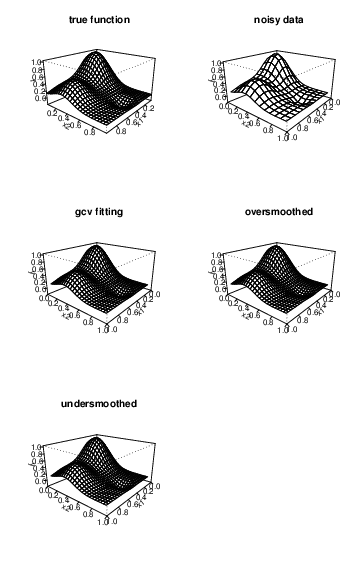
\includegraphics[scale=0.8]{result_0001.png}

            \caption{Results from $\sigma = 0.001m$.}

            \end{centering}
        \end{figure}

        \begin{figure}[!ht]
            
            \begin{centering}
                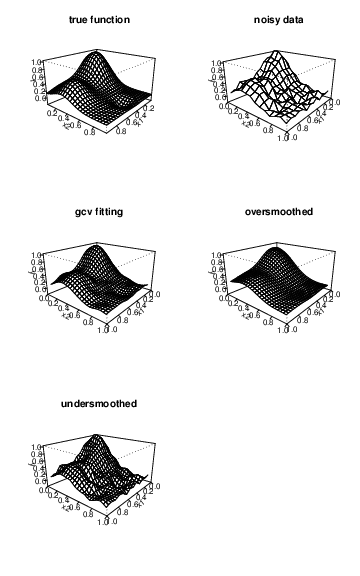
\includegraphics[scale=0.8]{result_006325.png}

            \caption{Results from $\sigma = 0.006235m$.}

            \end{centering}
        \end{figure}
        \begin{figure}[!ht]
            
            \begin{centering}
                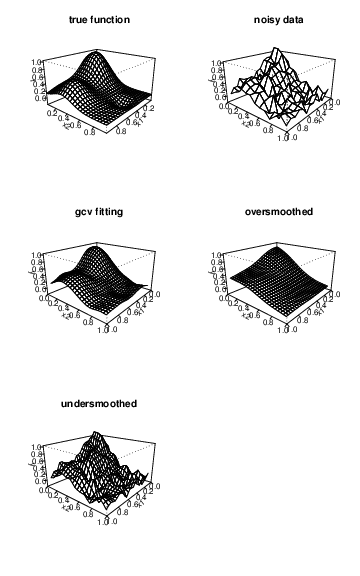
\includegraphics[scale=0.8]{result_01255.png}

            \caption{Results from $\sigma = 0.01255m$.}

            \end{centering}
        \end{figure}

        \begin{figure}[!ht]
            
            \begin{centering}
                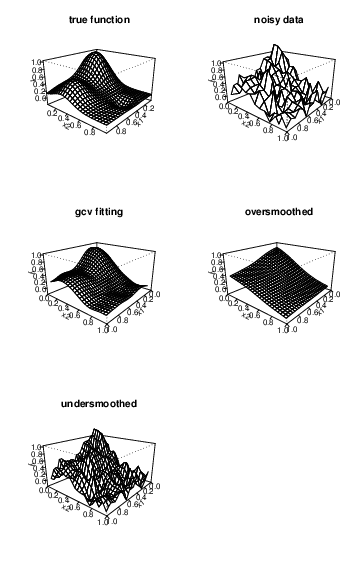
\includegraphics[scale=0.8]{result_018775.png}

            \caption{Results from $\sigma = 0.018775m$.}

            \end{centering}
        \end{figure}

        \begin{figure}[!ht]
            
            \begin{centering}
                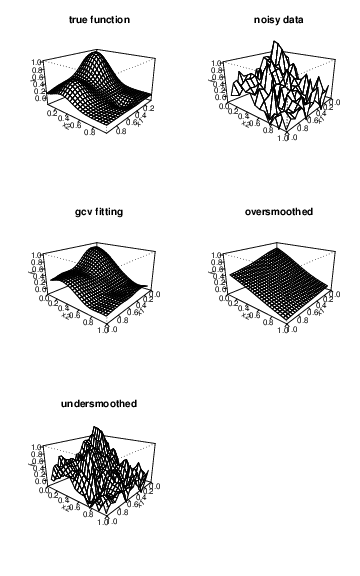
\includegraphics[scale=0.8]{result_025.png}

            \caption{Results from $\sigma = 0.025m$.}

            \end{centering}
        \end{figure}



\end{homeworkProblem}
%===============================================================================


\end{document}

